\section*{Glossaire}
\markboth{GLOSSAIRE}{GLOSSAIRE}
\addcontentsline{toc}{section}{Glossaire}


- \textbf{Algorithme :} Un ensemble de règles que la machine suit pour atteindre un objectif particulier. Un algorithme peut être considéré comme une recette qui définit les entrées, la sortie et toutes les étapes nécessaires pour passer des entrées à la sortie.

- \textbf{Apprentissage Automatique :} Un ensemble de méthodes permettant aux ordinateurs d'apprendre à partir de données pour faire et améliorer des prédictions (par exemple le cancer, les ventes hebdomadaires, le défaut de crédit).

\begin{center}
    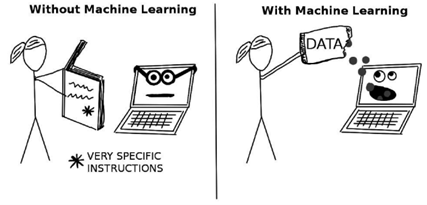
\includegraphics[width=0.7\linewidth]{Images/ml_illustration.png}
    \\
    \textbf{Figure 1:} Illustration d'aide à la compréhension du concept de ML 
\end{center}

- \textbf{Apprenant ou Algorithme d'Apprentissage Automatique :} Le programme utilisé pour apprendre un modèle d'apprentissage automatique à partir de données. Un autre nom est "inducteur" (par exemple "inducteur d'arbre").

- \textbf{Modèle d'Apprentissage Automatique :} Le programme appris qui relie les entrées aux prédictions. Cela peut être un ensemble de poids pour un modèle linéaire ou pour un réseau neuronal.

- \textbf{Modèle Boîte Noire :} Un système qui ne révèle pas ses mécanismes internes. En apprentissage automatique, "boîte noire" décrit les modèles qui ne peuvent pas être compris en regardant leurs paramètres (par exemple un réseau neuronal). L'opposé d'une boîte noire est parfois appelé Boîte Blanche et est décrit dans ce livre comme modèle interprétable.

- \textbf{Apprentissage Automatique Interprétable :} Se réfère aux méthodes et modèles qui rendent le comportement et les prédictions des systèmes d'apprentissage automatique compréhensibles pour les humains.

- \textbf{Instance :} Une ligne dans l'ensemble de données.

- \textbf{Caractéristiques :} Les entrées utilisées pour la prédiction ou la classification. Une caractéristique est une colonne dans l'ensemble de données.

- \textbf{Cible :} L'information que la machine apprend à prédire.

- \textbf{Tâche d'Apprentissage Automatique :} La combinaison d'un ensemble de données avec des caractéristiques et une cible. Selon le type de la cible, la tâche peut être par exemple la classification, la régression, l'analyse de survie, le regroupement ou la détection d'anomalies.

- \textbf{Prédiction :} Ce que le modèle d'apprentissage automatique "devine" comme valeur cible en fonction des caractéristiques données.

